\section{Preliminaries}\label{Section:Preliminaries}
%Preliminaries for the temporal series data analysis: correlograms, partial correlograms. %Preliminaries for the AMIDST models.

\subsection{Dynamic Bayesian Networks}

\begin{figure}
\begin{center}
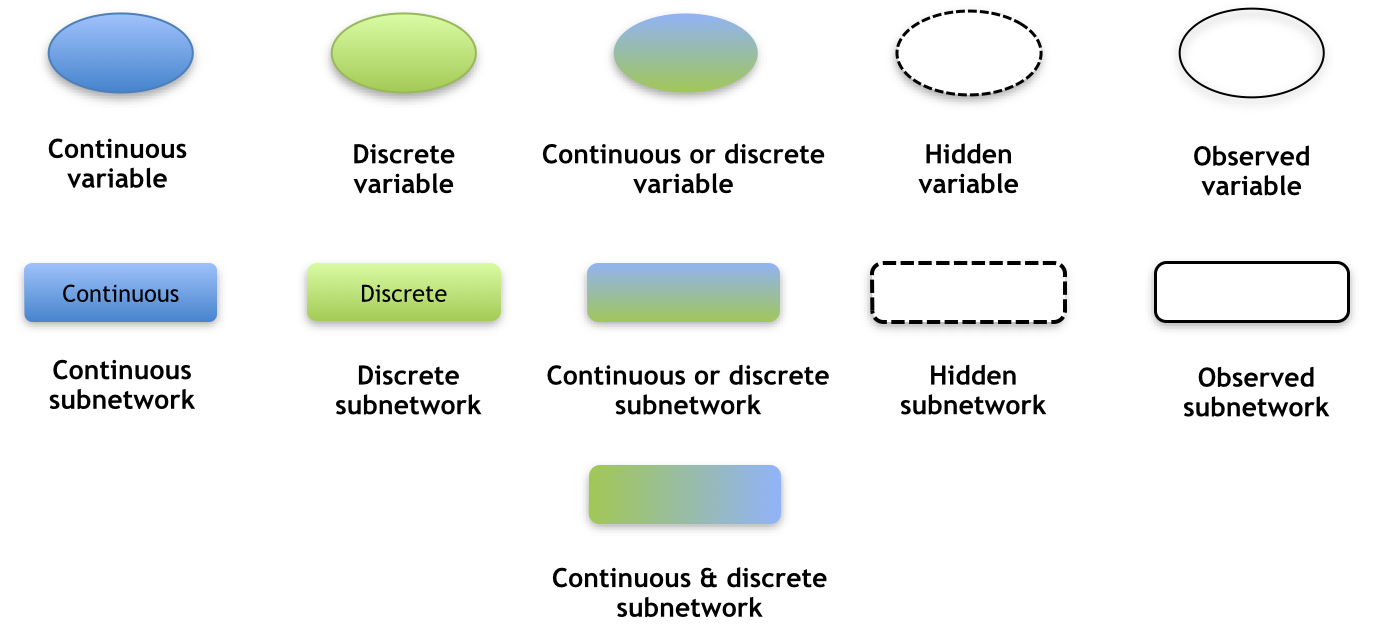
\includegraphics[scale=0.4]{./figures/PreliminariesNotation}
\caption{\label{Figure:Preliminaries Notation}PreliminariesNotation
}
\end{center}
\end{figure}

\subsection{Data analysis}

As already commented in the introduction, the data analysis detailed here will be used to test some assumptions supporting the models elicited by the experts in the different use cases, and also to complement our understanding about the nature of the problem we are modelling. The set of tools employed for this purpose allow us to get insights about some simple and basic aspects of the structural and the distributional assumptions present in a dynamic Bayesian network (DBN).

\subsubsection*{Structural assumptions: sample correlograms and partial correlograms}

A DBN mainly aims to model complex multivariate time series. By using sample correlogramas and sample partial correlograms, we will try to test if the available data supports the temporal correlation between variables assumed by the DBN model, i.e., the temporal links between variables. However, these tools will only allow us to look at univariate time series, what strongly limits the reach of the  extracted conclusions. But, at least and as we will see later in the different use-cases, this analysis will give us some interesting insights which usually can not be elicited from experts.  

\begin{description}
\item[Sample correlogram:] Let ${x_1,...,x_T}$ be a univariate time series. The \emph{sample autocorrelation coefficient} at lag $v$ is given by 

$$ \hat{\rho}_v =\frac{\sum_{t=1}^{T-v} (x_t-\bar{x})(x_{t+v}-\bar{x})}{\sum_{t=1}^{n} (x_t-\bar{x})^2}$$ 

\noindent where $\bar{x}$ is the sample mean. The plot of $\hat{p}_v$ versus $v$ for $v=1,..., M$ for some maximum $M$ is called the \emph{sample correlogram} of the data.

\item[Sample partial correlogram:] Let us denote by $X_t$ to the random variable associated to $X$ taking values at time $t$. We can build the following regression problem:

$$ X_t = a_0 + a_1X_{t-1} + a_2X_{t-2} + ... a_{v-1}X_{t-v-1}$$

In addition, let $e_{i,v}$ denotes the residuals of this regression problem (i.e., the error when estimating $X_t$ using a linear combination of $v-1$ previous observations). The \emph{sample partial autocorrelation coefficient} of lag $v$, denoted as  $\hat{\theta}_v$, is the standard sample autocorrelation between  the variable $X_{t-v}$ and these residuals. Intuitively, the sample partial autocorrelation coefficient of lag $v$ can be seen as the correlation between $X_t$ and $X_{t+v}$ after having removed the common \emph{linear} effect of the data in between.
\end{description}

Sample correlograms can be interpreted as a way to measure the strength of the following unconditional dependences: $X_t  \not\perp X_{t+v}$ for some lag $v \geq 1$.  When $\hat{\rho}_v$ is close to zero, this strongly indicates that there is an unconditional independence between $X_t$ and $X_{t+v}$. However, when $\hat{\rho}_v$ is close to either $1$ or $-1$, this strongly indicates that there is a correlation or dependency between $X_t$ and $X_{t+v}$. But, again, we should never forget that we are making linear relationships and normality assumptions. 

Figure \ref{Figure:PreliminariesCorrelograms} shows an example of how a sample correlogram looks like for two kind of data sets: First, a sequence of 50 data samples i.i.d. according to a Gaussian distribution with zero mean and unit variance $x_t\sim N(0,1)$ (see Figure \ref{Figure:PreliminariesCorrelograms}(a));  and second, a sequence of 50 data samples distrubuted as $x_t=x_{t-1} + \epsilon$, $x_0=\epsilon$, such that $\epsilon\sim N(0,1)$ (see  Figure \ref{Figure:PreliminariesCorrelograms}(b)). As can be seen, for the i.i.d. data the correlogram has always values close to zero for all the lags. However, for time series data, the correlogram clearly identifies the presence of a temporal relationship in the data. As expected, the correlation decreases with the size of the lag, and how quickly it decreases depends on the strength of the temporal relationship. 

Similarly, we plot in Figure \ref{Figure:PreliminariesCorrelograms}(c) and  in  Figure \ref{Figure:PreliminariesCorrelograms}(d) the sample partial correlograms for the same two data sequences presented above. In the case of i.i.d. data, we can see again that the partial correlogram does not show any sign of partial correlation between the data sequence samples. However, for time series data, the partial correlogram takes a high value for $v=1$ and then is null for $v$ higher than 1. Sample partial correlogram can be interpreted as a way to measure the strength of the following conditional dependence: $X_t  \not\perp X_{t+v} | X_1,...,X_{t+v-1}$ for some lag $v\geq 1$.  Accordingly, the sample partial correlogram correctly identifies that we have the following conditional independencies: $X_t\perp X_{t+2}|X_{t+1}$ in the considered time series data. Therefore, sample partial correlogram can be seen as a tool to test the order of the Markov chain generating a time data sequence, with all the same caveats expressed for the sample correlogram. 

\begin{figure}
\begin{center}
\begin{tabular}{cc}
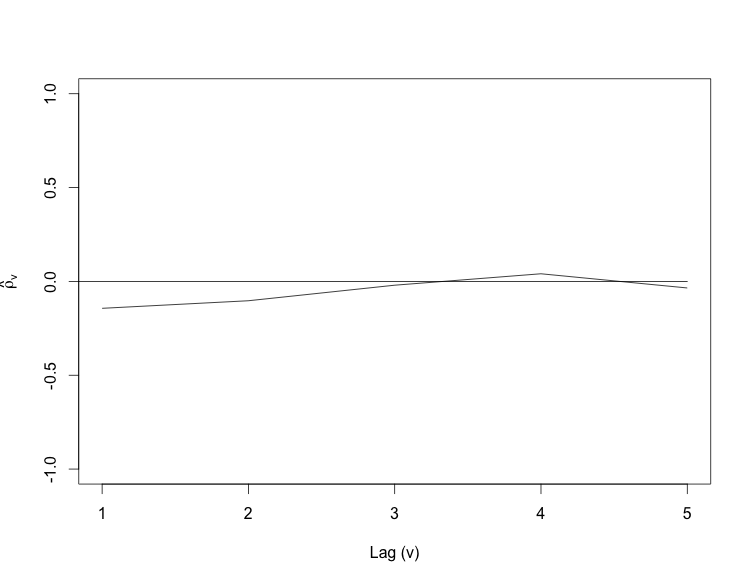
\includegraphics[scale=0.25]{./figures/CorrelogramGaussian} &
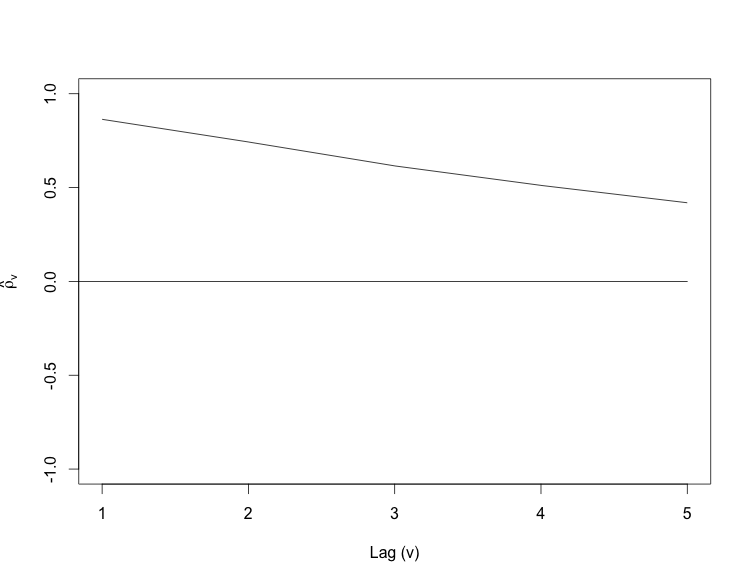
\includegraphics[scale=0.25]{./figures/CorrelogramTimeSerie} \\
(a) Correlogram for i.i.d. data & (b) Correlogram for a time series data \\
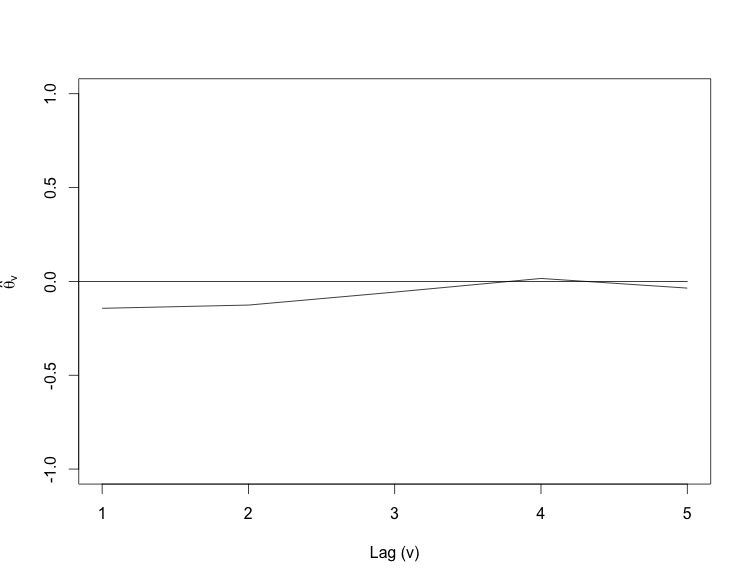
\includegraphics[scale=0.25]{./figures/PartialCorrelogramGaussian} &
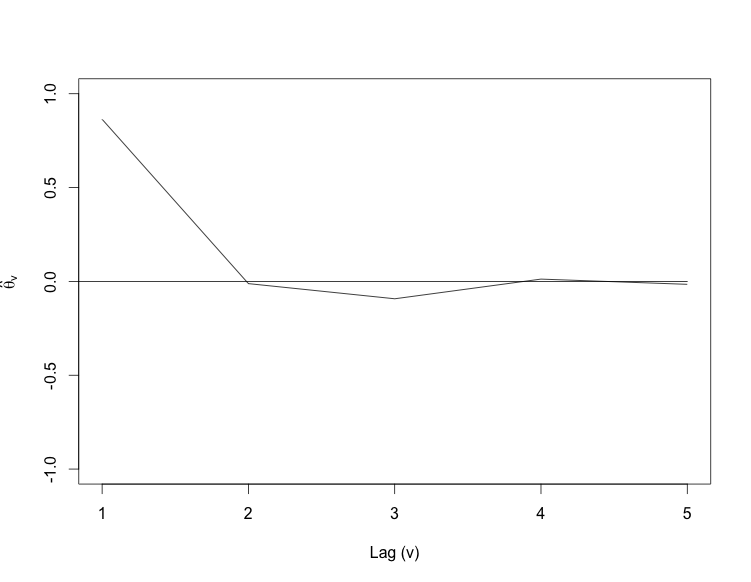
\includegraphics[scale=0.25]{./figures/PartialCorrelogramTimeSerie} \\
(c) Partial correlogram for i.i.d. data & (d) Partial correlogram for a time series data \\
\end{tabular}
\caption{\label{Figure:PreliminariesCorrelograms} Examples of sample correlograms and sample partial correlograms for i.i.d. and time series data. 
}
\end{center}
\end{figure}

\subsubsection*{Distributional assumptions: Histograms and Bivariate Distributions}

With the tools described in this section we tried to get insights about the conditional distribution probabilities  of the proposed models. The first basic tool that we employed for this purpose was the histograms. However this tool, although quite useful in a static context, is quite limited in dynamic models. For example, let assume we have a time series $x_1,\ldots, x_T$ and our histogram shows that the empirical distribution of the variable when we aggregate the data samples over time looks like a mixture of Gaussian distributions. There are two simple possibilities that can give rise to this finding: i)  $X_t$ is distributed according to a mixture of Gaussians where each Gaussian component depends on $X_{t-1}$; ii) there is a discrete hidden variable that influences $X_{t}$ but which is not observed and it is the one that generates the different mixture components.  As shown in this example, histograms are difficult to interpret in dynamic models, but we are going to use them when we think that they can be of some help. 

The other tool that we are going to use to get insights about the conditional distributions of the model is the contour plot of the empirical bivariate distribution of $X_t$ versus $X_{t-1}$.  These contour plots can show many relevant information such as if there are linear relationships between variables or if we can assume they are normality distributed, etc. In Figure \ref{Figure:PreliminariesBivariates}, we plot the bivariate contour plot for the i.i.d data and the time series data previously employed when describing the sample correlograms. As can be seen, the bivariate contour plot of the time series clearly show a linear relationship between $X_t$ and $X_{t-1}$  and how they can be assumed to be distributed according to a bivariate normal with a covariance that displays some degree of correlation. In the case of i.i.d. data, the contour plot looks like quite different. 

\begin{figure}
\begin{center}
\begin{tabular}{cc}
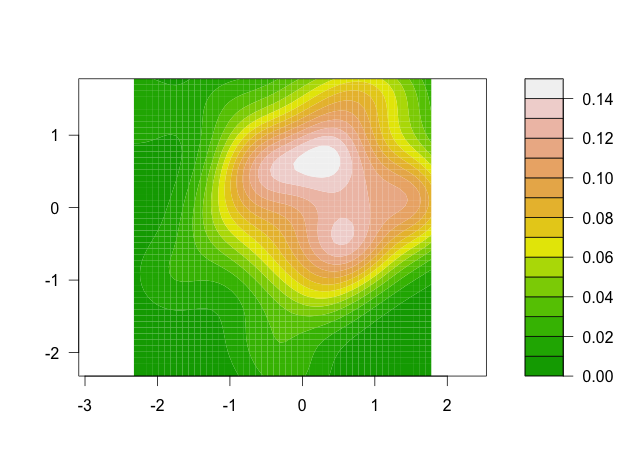
\includegraphics[scale=0.25]{./figures/BivariateGaussian} &
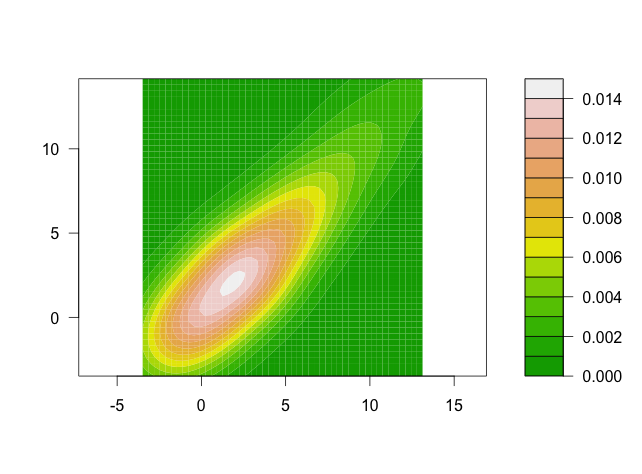
\includegraphics[scale=0.25]{./figures/BivariateTimeSerie} \\
(a) i.i.d. data & (b)  Time series data \\
\end{tabular}
\caption{\label{Figure:PreliminariesBivariates}Bivariate contour plots for a set of i.i.d. data and for a time series data. 
}
\end{center}
\end{figure}


>>>>>>> 4b6c554498b8852b9e3f137d4e4d563e21672013
